% \chapter{Implementasi dan Pengujian}
\chapter{Rencana Pelaksanaan}

Bab ini berisikan rencana jadwal dan risiko yang berpotensi menghambat pengembangan rancangan solusi yang sudah diajukan pada Bab III.

% Bab Rencana Pelaksanaan digunakan untuk mendeskripsikan rencana pelaksanaan berupa jadwal dan risiko-risiko yang mungkin dihadapi dan rencana mitigasinya. Tujuan bab ini  adalah:
% 1.	Mahasiswa memiliki rencana yang jelas mengenai pelaksanaan TA
% 2.	Mahasiswa mengenali risiko-risiko yang mungkin dihadapi dan sudah menyiapkan diri untuk mengantisipasi risiko tersebut.

% \section{Lingkungan}
% \blindtext

% \section{Implementasi}
% \blindtext

% \section{Pengujian}
% \blindtext

\section{Jadwal}
\label{sec:jadwal}

% Cantumkan jadwal pengerjaan tugas akhir lengkap dengan uraiannya.

Jadwal pengerjaan Tugas Akhir ini dibagi menjadi beberapa tahap utama yang meliputi pengumpulan kebutuhan, perancangan solusi, pengembangan prototipe, dan pengujian prototipe. Setiap tahapan akan dilakukan dengan memperhatikan waktu yang dibutuhkan serta beberapa komponen tambahan seperti kegiatan akademik dan organisasi.

\begin{table}[h]
	\caption{Jadwal Pengerjaan Tugas Akhir}
	\vspace{0.25cm}
	\begin{center}
		\begin{tabular}{|c|l|c|l|}
			\hline
			\textbf{No} & \textbf{Tahapan}       & \textbf{Waktu} \\ \hline
			1           & Analisis Kebutuhan     & 1 minggu       \\ \hline
			2           & Perancangan Solusi     & 2 minggu       \\ \hline
			3           & Pengembangan Prototipe & 3 minggu       \\ \hline
			4           & Pengujian Prototipe    & 2 minggu       \\ \hline
			5           & Evaluasi dan Perbaikan & 1 minggu       \\ \hline
		\end{tabular}
	\end{center}
\end{table}

\begin{figure}[ht]
	\centering
	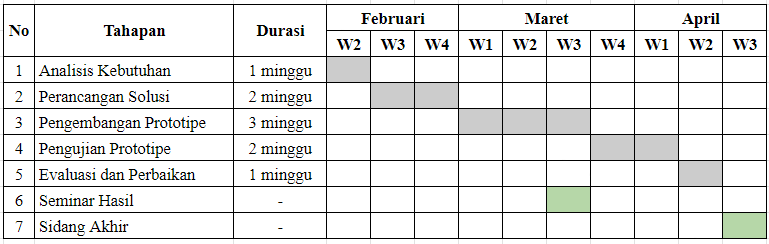
\includegraphics[width=1\textwidth]{resources/chapter-4/gantt-chart.png}
	\caption{Gantt Chart Jadwal Pengerjaan Tugas Akhir}
	\label{image:gantt-chart}
\end{figure}

Berikut merupakan penjelasan dari setiap tahapan pada jadwal pengerjaan Tugas Akhir:

\begin{enumerate}
	\item \textbf{Analisis Kebutuhan:} Tahap ini bertujuan mengidentifikasi kebutuhan sistem Smart Contract Discovery melalui studi literatur dan analisis fitur yang dibutuhkan. Hasil dari tahap ini berupa dokumen kebutuhan fungsional dan non-fungsional sebagai dasar perancangan.
	\item \textbf{Perancangan Solusi:} Tahapan ini mencakup desain arsitektur sistem, pemetaan data, dan pemilihan teknologi seperti eth2dgraph dan Dgraph. Fokus utamanya adalah mendefinisikan komponen sistem dan alur kerja yang akan diimplementasikan.
	\item \textbf{Pengembangan Prototipe:} Tahap ini melibatkan implementasi awal sistem, termasuk ekstraksi data smart contract, pengindeksan ke dalam Dgraph, dan pengembangan dasar mekanisme query untuk pencarian fungsionalitas.
	\item \textbf{Pengujian Prototipe:} Sistem diuji menggunakan dataset nyata atau simulasi untuk memastikan kinerja, akurasi, dan skalabilitas. Fokus pengujian adalah validasi fungsionalitas dan efisiensi sistem.
	\item \textbf{Evaluasi dan Perbaikan:} Evaluasi dilakukan untuk mengidentifikasi kelemahan dan perbaikan sistem berdasarkan hasil pengujian. Tahap ini memastikan sistem berfungsi optimal sesuai kebutuhan.
	      % \item \textbf{Seminar Hasil}: Memaparkan hasil dari progress pengembangan prototipe, beserta analisis dan hasil yang ditemukan sampai proses pengembangan prototipe.
	      % \item \textbf{Sidang Akhir}: Memaparkan hasil dari Tugas Akhir, prototipe yang dikembangkan, dan juga hasil analisis
\end{enumerate}

\section{Risiko}
\label{sec:risiko}

% misal kegiatan apa yang akan jadi tantangan, misal ada kepengurusan, jadi lebih baik dituliskan agar diperhatikan
% misal kurang banyak artikel yang dituliskan

% Cantumkan 5 risiko tertinggi yang mungkin dihadapi dalam pengerjaan tugas akhir. Risiko yang dicantumkan dapat merupakan risiko dari sisi teknis, risiko dari sisi operasional, risiko dari metode yang dipilih, dan sebagainya. Cantumkan pula rencana mitigasi dari risiko-risiko tersebut.

Tugas Akhir ini memiliki beberapa risiko yang mungkin mempengaruhi kelancaran pengerjaan. Risiko tersebut melibatkan faktor teknis, operasional, metodologis, dan pribadi. Berikut adalah lima risiko tertinggi beserta rencana mitigasinya:

\begin{enumerate}
	\item \textbf{Kompleksitas Implementasi Sistem (Teknis)} \newline
	      Deskripsi: Implementasi sistem Smart Contract Discovery, terutama pada aspek \textit{semantic enrichment} dan pengintegrasian dengan Dgraph, dapat menghadapi tantangan teknis, terutama terkait pemrosesan data besar dan pembuatan query yang efisien. \newline
	      Mitigasi:
	      \begin{enumerate}
		      \item Melakukan riset mendalam dan uji coba modul secara bertahap.
		      \item Menggunakan \textit{dokumentasi} dari eth2dgraph dan komunitas Dgraph untuk mempercepat pemahaman tentang teknis implementasi.
		      \item Mempersiapkan \textit{prototipe modular} yang mudah untuk diuji coba dan dikembangkan.
	      \end{enumerate}
	\item \textbf{Kurangnya Referensi Terkait Topik Spesifik (Metodologi)} \newline
	      Deskripsi: Tidak banyak artikel yang secara spesifik membahas tentang smart contract discovery systems dan penerapan semantic indexing pada blockchain yang berskala besar.  \newline
	      Mitigasi:
	      \begin{enumerate}
		      \item Memfokuskan pencarian pada literatur yang relevan meskipun tidak langsung membahas topik ini secara keseluruhan.
		      \item Menggunakan berbagai sumber alternatif seperti makalah konferensi, whitepapers, dan riset terkait di bidang blockchain dan semantic technologies.
	      \end{enumerate}
	\item \textbf{Kesulitan dalam Pemetaan dan Klasifikasi Fungsionalitas Smart Contracts (Metodologi)}  \newline
	      Deskripsi: Pemetaan dan pelabelan fungsionalitas smart contracts secara semantik dapat menjadi tantangan besar, terutama pada data yang tidak terdokumentasi dengan baik. \newline
	      Mitigasi:
	      \begin{enumerate}
		      \item Menggunakan teknik \textit{machine learning} atau \textit{NLP} untuk otomatisasi pelabelan fungsionalitas.
		      \item Melakukan validasi manual pada data yang tidak terdokumentasi dengan baik.
	      \end{enumerate}
	\item \textbf{Batasan Kapasitas Mesin yang Digunakan dalam Pengembangan (Operasional)} \newline
	      Deskripsi: Pengembangan solusi dalam ranah Blockchain membutuhkan sebuah mesin yang dapat memproses data yang banyak dan memiliki penyimpanan yang besar. \newline
	      Mitigasi:
	      \begin{enumerate}
		      \item Menggunakan penyimpanan eksternal untuk menyimpan data yang besar
		      \item Menggunakan mesin yang memiliki kapabilitas pemrosesan yang lebih kuat
	      \end{enumerate}
	\item \textbf{Stres dan Tekanan dari Banyaknya Tanggung Jawab (Pribadi)}  \newline
	      Deskripsi: Beban tugas dan tanggung jawab yang banyak dapat menyebabkan stres dan mempengaruhi kualitas pengerjaan tugas akhir. Tanggung jawab seperti kepengurusan organisasi sampai bulan Mei, kewajiban akademik berupa pengambilan beberapa mata kuliah dan juga pekerjaan magang yang dikerjakan dapat menumpuk tekanan. \newline
	      Mitigasi:
	      \begin{enumerate}
		      \item Melakukan \textit{time management} yang baik, dan ambil waktu untuk beristirahat.
		      \item Mempertimbangkan delegasi tugas organisasi kepada anggota yang kompeten.
	      \end{enumerate}
\end{enumerate}